\documentclass[a4paper,onesided,12pt]{report}
\usepackage{styles/fbe_tez}
\usepackage[utf8x]{inputenc} % To use Unicode (e.g. Turkish) characters
\renewcommand{\labelenumi}{(\roman{enumi})}
\usepackage{amsmath, amsthm, amssymb}
 % Some extra symbols
\usepackage[bottom]{footmisc}
\usepackage{cite}
\usepackage{graphicx}
\usepackage{longtable}
\graphicspath{{figures/}} % Graphics will be here

\usepackage{multirow}
\usepackage{subfigure}
\usepackage{algorithm}
\usepackage{algorithmic}
%\pagestyle{empty}
%\includeonly{introduction} % To only process the given file

\newtheorem{thm}{Theorem}[chapter]
\newtheorem{prop}[thm]{Proposition}
\newtheorem{lem}[thm]{Lemma}
\newtheorem{cor}[thm]{Corollary}
% COVER PAGE
\title{EMPOWERING HETEROGENEOUS NETWORKS FOR DRUG-TARGET AFFINITY PREDICTION}
\turkcebaslik{\.{I}LA\c{C}-HEDEF BA\u{G}LILIK \.{I}LG\.{I}S\.{I} TAHM\.{I}N\.{I} \.{I}\c{C}\.{I}N HETEROJEN A\u{G}LARI GÜ\c{C}LEND\.{I}RME }
\degree{B.S., Computer Engineering, Marmara University, 2018\\
	M.S., Computer Engineering, Boğaziçi University, 2021}
\author{Selen Parlar}
\program{Computer Engineering}
\subyear{2021}

% APPROVED BY PAGE
\supervisor{Assoc. Prof. Arzucan \"{O}zg\"{u}r}
%\cosuperi{Title and Name of Cosupervisor I}
%\cosuperii{Title and Name of Cosupervisor II}
% \examineri{Assist. Prof. H. Birkan Y{\i}lmaz}
% \examinerii{Assist. Prof. \"{O}znur Ta\c{s}tan}
\examineri{Name Surname, Ph.D.}
\examineri{Name Surname, Ph.D.}
%\examineriv{}
%\examinerv{}
\dateofapproval{DD.MM.YYYY}


\begin{document}

\pagenumbering{roman}
\makemstitle % M.S. thesis
\makeapprovalpage
\begin{acknowledgements}
Acknowledgements come here...
\end{acknowledgements}
\begin{abstract}
One page abstract will come here.  
\end{abstract}
\begin{ozet}
Bir sayfa uzunluğunda özet gelecektir.
\end{ozet}
\tableofcontents
\listoffigures
\listoftables
\begin{symbols}
% The title will be typeset as "LIST OF SYMBOLS".
%
% Use a separate \sym command for each symbols definition.
% First Latin symbols in alphabetical order

\sym{$a_{ij}$}{Description of $a_{ij}$}
\sym{$\mathbf{A}$}{State transition matrix of a hidden Markov model}
% Then Greek symbols in alphabetical order
\sym{}{}
\sym{$\alpha$}{Blending parameter \textit{or} scale}
\sym{$\beta_t(i)$}{Backward variable}
\sym{$\Theta$}{Parameter set}
\sym{ }{}

\end{symbols}

\begin{abbreviations}
 % Abbreviations in alphabetical order
\sym{2D}{Two Dimensional}
\sym{3D}{Three Dimensional}
\sym{AAM}{Active Appearance Model}
\sym{ASM}{Active Shape Model}
\end{abbreviations}


\chapter{INTRODUCTION}
\label{chapter:introduction}
\pagenumbering{arabic}
Drug design is an expensive and time-consuming process that can be carried out by testing the existing chemicals on different types of protein targets \cite{csermely2013structure}. Furthermore, drug design is a highly dynamic field due to the continuous evolution of target proteins and their different responses to the same drugs over time. During the process, several factors are considered such as protein-ligand binding affinity, bioactive conformation, pharmacokinetic parameters, metabolic stability, selectivity, toxicity, and synthesizability.

The main goal of drug design is to provide a selective effect while minimizing the side-effects by targeting only the disease-specific receptors and protecting the healthy cells. Today, rational designs that save time and cost in the pharmaceutical design are applied and it is possible to develop drugs with selectively effective and fewer side effects. This rational discovery process often begins with the development of a drug active substance, by selecting and improving ligands from a molecule library. However, the size of the drug search space is huge when we consider the existence of 97 million chemicals in the chemical database PubChem \cite{bolton2008pubchem} and the 16,526 drugs in the DrugBank \cite{law2013drugbank}. Due to the expansive search space, the need for computational methods has emerged for this multi-stage, trial and error based process. 

Computational methods aim to determine the interacting and non-interacting drug and target pairs, and binary classification methods have been commonly used \cite{yamanishi2010drug, liu2016neighborhood, nascimento2016multiple, keum2017self, greenside2017prediction}. Binary classification-based approaches provide information about a possible interaction between proteins and ligands, however, the strength of the protein-ligand interactions, namely the binding affinity, cannot be determined with these methods. Binding affinity is important  in the drug design pipeline since a strong interaction is the first step in finding a selective drug. However, prediction of the binding affinity value still remains a challenge \cite{ozturk2018deepdta}. In this thesis, we propose a graph-based model to predict the drug target binding affinities.
% Continue with the actual proposal
%Start with an introduction...
\chapter{RELATED WORK}
\label{related_work}

<<<<<<< Updated upstream
=======
<<<<<<< HEAD
The computational methods used in drug discovery recently focused on four strategies; ligand similarity-based \cite{keiser2007relating}, molecular docking/structure-based \cite{morris2009autodock4,donald2011algorithms}, deep learning-based \cite{wan2018neodti, luo2017network}, and network-based approaches \cite{luo2017network, zheng2013collaborative, chen2012drug, wang2014drug}. The performance of the ligand similarity-based approaches is often low when a target has a few known binding ligands. Also, the limited availability of 3D structures of target proteins limits the molecular docking performance. Due to the limited data availability, some efforts have been devoted to developing machine learning-based approaches for drug target affinity (DTA) predictions through computational techniques. The growing amount of drug-target binding affinity data available in online databases has led to the adoption of advanced learning techniques such as deep learning architectures in predicting binding affinities \cite{chan2016large, tian2016boosting, hamanaka2017cgbvs, ozccelik2021chemboost, ozturk2018deepdta, ozturk2019widedta}. Last but not least, with networks, the ability to integrate several types of information, the affinity prediction task gained some other insights, and in the last decade, the number of studies increased \cite{wan2018neodti, luo2017network, nguyen2019graphdta}.

%Protein-ligand scoring is used to approximately predict the binding affinity between two molecules, and it is frequently used after the virtual screening, and docking campaigns \cite{ragoza2017protein}. One of the successful alternative machine learning methods to scoring functions is the Random Forest algorithm \cite{ballester2010machine, shar2016pred}. However, it fails in virtual screening and docking tests due to oversimplification of the protein-ligand complex descriptions \cite{gabel2014beware}. The continuously expanding amount of protein-ligand binding data enables deep learning methods in scoring. For instance, 3D structures of protein-ligand complexes are commonly used with Convolutional Neural Networks (CNNs) \cite{gomes2017atomic, ragoza2017protein, wallach2015atomnet}; however, its success is limited to known protein-ligand complex structures. Kronecker Regularized Least Squares (KronRLS) algorithm is also used in scoring \cite{pahikkala2014toward}. Only 2D compound similarity-based drug representations and Smith-Waterman similarity representations of the targets are used in KronRLS. Another approach proposed to predict the binding affinity scores is SimBoost method \cite{he2017simboost}. It uses a gradient boosting machine with extracted features from drug-target pairs' interactions and similarity-based information. 

Several types of deep learning frameworks have been adopted in the DTA prediction task. DeepDTA \cite{ozturk2018deepdta} and WideDTA \cite{ozturk2019widedta} approaches are proposed to predict the binding affinities of protein-ligand interactions. Both methods utilize deep learning models that use only 1D representations of proteins and ligands. As the 1D representation, both studies use SMILES (Simplified Molecular Input Line Entry System) representations of the compounds rather than complex external features. DeepDTA learns high dimensional features from full-length sequences of the proteins and ligands. It uses two Convolutional Neural Networks (CNNs) to learn the representations of drugs and proteins. Then, the concatenated representations of drugs and proteins are fed into a multi-layer perceptron (MLP). 
Nevertheless, it fails to capture the biologically important short subsequences. WideDTA overcomes this problem by integrating different kinds of text-based information such as protein sequence, ligand SMILES, protein domains and motifs, and maximum common substructure words to provide better representation and predict binding affinity. To do that, WideDTA employs four CNNs and learns the representations of drugs and proteins. 
Similarly, it uses the MLP with the concatenated representations. The DeepConv-DTI \cite{lee2019deepconv} also utilizes CNNs on the protein sequences. On the other hand, they use 2D structural images of chemicals to learn complex features using CNNs and produce DTA predictions.

Although the extensive experiments and enhanced performance in the DTA prediction task, representing the drugs as strings cause a loss of information since 1D representations cannot fully represent the structural information beneath the biomolecules. Graph neural networks (GNNs) are employed to address this problem, and drugs are represented as graphs. Tsubaki \textit{et al.} \cite{tsubaki2019compound} propose to use CNNs and GNNs together to learn the representation of compound graphs and protein sequences. They demonstrate performance improvement on the DTA task compared to the feature-based methods. GraphDTA \cite{nguyen2019graphdta} also suggests a new neural network architecture for the drug-target affinity prediction task. Rather than using the 1D representation of SMILES, they convert SMILES representation into a molecular graph and employ a graph neural network (GNN) to learn a graph representation. Moreover, they encode and embed protein amino acid sequences and use CNN to create protein representations. Then, combine CNNs and GNNs to predict the binding affinity value. Another method, DGraphDTA \cite{jiang2020drug}, uses graphs to represent both compounds and proteins with GNNs. Additionally, to address the interpretability, several models employ an attention mechanism \cite{karimi2020explainable, chen2020transformercpi, agyemang2020multi, yang2021ml}. 

Rather than using only the known drug-target interaction (DTI) data in deep learning models, some other diverse information from heterogeneous data sources integrated into the systems, such as protein-protein interaction (PPI), drug-disease association, drug-side effect association as in the work of MSCMF \cite{zheng2013collaborative}, HNM \cite{wang2014drug}, DTINet \cite{luo2017network}, and NeoDTI \cite{wan2018neodti}. They employ networks that can capture the complex relationships between different types of components, such as drugs and proteins. These methods have improved the performance in the DTI prediction task, yet they have some limitations to be addressed. For instance, in MSCMF \cite{zheng2013collaborative}, drug and protein similarity matrices are gathered from different data sources via a weighted averaging scheme in order to use in the matrix factorization of a given DTI network. However, this data integration often causes data loss, resulting in a suboptimal solution. Moreover, DTINet \cite{luo2017network} is developed as a computational pipeline to predict novel DTI from a heterogeneous network. First, it learns low-dimensional feature representations of drugs and targets in an unsupervised manner. Then it predicts new DTIs with inductive matrix completion (IMC) as in the work of Natarajan and Dhillon \cite{natarajan2014inductive}. Since DTINet handles the unsupervised feature learning procedure and the prediction task separately, it may cause non-optimal solutions. NeoDTI \cite{wan2018neodti} targets this problem and combines feature learning and classification into a single task, improving the accuracy. 

More recently, Zhao \textit{et al.} \cite{zhao2021identifying} propose a method that combines GNNs and deep neural networks (DNNs) for the DTI prediction task. They build a drug-protein network using drug-drug interaction, protein-protein interaction, and drug-protein interaction networks in which nodes represent drugs and proteins, and edges represent the link strength between them. Then, handles the DTI prediction problem as a node classification problem. Another network-based method EEG-DTI \cite{peng2021end} proposes an end-to-end heterogeneous graph representation learning-based framework to predict the interaction between drugs and targets using graph convolutional networks (GCNs). DTiGEMS$+$ \cite{thafar2020dtigems+} constructs a heterogeneous graph using the DTI graph with drug-drug similarity and target-target similarity graphs. It combines feature-based and similarity-based approaches to model the identification of drug-target pairs. After performing graph augmentation, it applies node2vec \cite{grover2016node2vec} for feature representation learning of drugs and targets and uses them in a link prediction task. To improve the DTiGEMS$+$'s performance, DTi2Vec \cite{thafar2021dti2vec} is proposed in which representation learning and ensemble learning techniques are combined to identify the drug-target interactions. Unlike the previous work, it uses edge embeddings between drug-target node pairs rather than node embeddings. Given the success of heterogeneous graphs in the DTI prediction and text-based methods in DTA prediction, in this thesis, we propose a method for DTA prediction that utilizes heterogeneous graphs together with the biomolecular language-based information obtained from the text representations of chemicals and proteins. 
%This is the first study that combines heterogeneous graphs and biomolecular language-based information for the DTA prediction task to the best of our knowledge. 

% Yine biraz karisiklik var. Metotlari detayli anlatmissin. Emege saygi +rep. Ama genel cerceveden kopmak cok kolay oluyor okurken. Arada olaylari birbirine baglamak ve neyi neden anlattigina dair bir seyler yazmak iyi olabilir.

% Karisik pargraflari toplamak icin bkz: tek cumlelik ozet
=======
>>>>>>> Stashed changes
Traditional computational methods used in drug discovery are based on four strategies; ligand similarity-based \cite{keiser2007relating}, molecular docking/structure-based \cite{morris2009autodock4,donald2011algorithms}, deep learning-based \cite{wan2018neodti, luo2017network}, and network-based approaches \cite{luo2017network, zheng2013collaborative, chen2012drug, wang2014drug}. The performance of the ligand similarity-based approaches is often low when a target has a few known binding ligands. Likewise, the limited availability of 3D structures of target proteins limits the molecular docking performance. In the last decade, some effort has been devoted to developing machine learning-based approaches for drug target affinity (DTA) predictions through computational techniques. Binding affinity provides information on the strength of the interaction between a drug-target pair and the increase in available affinity data in online databases has led to the use of advanced learning techniques such as deep learning architectures in predicting binding affinities \cite{chan2016large, tian2016boosting, hamanaka2017cgbvs}.

Protein-ligand scoring is used to approximately predict the binding affinity between two molecules, and it is frequently used after virtual screening and docking campaigns \cite{ragoza2017protein}. One of the successful alternative machine learning methods to scoring functions is Random Forest algorithm \cite{ballester2010machine, shar2016pred}. However, it fails in virtual screening and docking tests due to oversimplification of the protein-ligand complex descriptions \cite{gabel2014beware}. The continuously expanding amount of protein-ligand binding data enables the use of deep learning methods in scoring. For instance, 3D structures of protein-ligand complexes are commonly used with Convolutional Neural Networks (CNNs) \cite{gomes2017atomic, ragoza2017protein, wallach2015atomnet}, however, its success is limited to known protein-ligand complex structures. Kronecker Regularized Least Squares (KronRLS) algorithm is also used in scoring \cite{pahikkala2014toward}. It utilizes only 2D based compound similarity-based representations of the drugs and Smith-Waterman similarity representation of the targets. Another approach proposed to predict the binding affinity scores is SimBoost method \cite{he2017simboost}. It uses a gradient boosting machine with the extracted features from interactions between drug-target pairs and their similarity-based information. 

Several types of deep learning frameworks have been adopted in DTA prediction task. DeepDTA \cite{ozturk2018deepdta} and WideDTA \cite{ozturk2019widedta} approaches are proposed to predict the binding affinities of protein-ligand interactions. Both methods utilize deep learning models that use only 1D representations of proteins and ligands. As the 1D representation, both of the studies use SMILES (Simplified Molecular Input Line Entry System) representations of the compounds rather than complex external features or 3D-structures of the binding complexes. DeepDTA learns high dimensional features from full-length sequences of the proteins and ligands. It uses two CNNs to learn the representations of drugs and proteins. Then, the concatenated representations of drugs and proteins are fed into the a multi-layer perceptron (MLP). Yet, it fails to capture the biologically important short subsequences. WideDTA overcomes this problem by integrating different kinds of text-based information such as protein sequence, ligand SMILES, protein domains and motifs, and maximum common substructure words to provide better representation and to predict binding affinity. To do that, WideDTA employs four CNNs and learn the representations of drugs and proteins. Similarly, uses the MLP with the concatenated representations. Lee \textit{et al.} \cite{lee2019deepconv} also utilizes CNNs on the protein sequences. On the other hand, they use 2D structural images of chemicals and learn complex features from them using CNNs and produce DTA predictions.

Although the extensive experiments and remarkable performance in DTA prediction task, representing the drugs as strings cause loss of information due to structural information lies beneath the molecules. To address this problem, graph neural networks (GNNs) are employed and drugs are represented as graphs. Tsubaki \textit{et al.} \cite{tsubaki2019compound} propose to use CNNs and GNNs together to learn the representation of compound graphs and protein sequences. They demonstrate performance improvement on DTA task compared to the feature-based methods. GraphDTA \cite{nguyen2019graphdta} also suggests a new neural network architecture for drug-target affinity prediction task. Rather than using the 1D representation of SMILES, they convert SMILES representation into a molecular graph and employ a graph neural network (GNN) to learn a graph representation. Moreover, they encode and embed protein amino acid sequences and use CNN to create protein representations. Then, combine CNNs and GNNs to predict the binding affinity value. Another method, DGraphDTA \cite{jiang2020drug}, uses graphs to represent both compounds and proteins and with GNNs. Additionally, to address the interpretability, several models employ attention mechanism \cite{karimi2020explainable, chen2020transformercpi, agyemang2020multi, yang2021ml}. 

Rather than using only the known drug-target interaction (DTI) data in deep learning models, some other diverse information from heterogeneous data sources integrated into the systems, such as protein-protein interaction (PPI), drug-disease association, drug-side effect association as in the work of MSCMF \cite{zheng2013collaborative}, HNM \cite{wang2014drug}, DTINet \cite{luo2017network}, and NeoDTI \cite{wan2018neodti}. They employ networks that are able to capture the complex relation between different types of components such as drugs and proteins. These methods have improved the performance in DTI prediction task, yet they have some limitations to be addressed. In MSCMF \cite{zheng2013collaborative}, drug and protein similarity matrices are gathered from different data sources via a weighted averaging scheme in order to use in matrix factorization of a given DTI network. However, this data integration often causes data loss that will result in a suboptimal solution. DTINet \cite{luo2017network} is developed as a computational pipeline to predict novel DTI from a heterogeneous network. First, it learns low-dimensional feature representations of drugs and targets with an unsupervised manner, then it predicts new DTIs with inductive matrix completion (IMC) as in the work of Natarajan and Dhillon \cite{natarajan2014inductive}. Since DTINet handles the unsupervised feature learning procedure and the prediction task separately, it may cause non-optimal solutions. NeoDTI \cite{wan2018neodti} targets this problem and combines feature learning and classification into a single task, improving the accuracy. 

More recently, Zhao \textit{et al.} \cite{zhao2021identifying} propose a method that combines GNNs and deep neural networks (DNNs) for DTI prediction task. They build a drug-protein network using drug-drug interaction, protein-protein interaction, and drug-protein interaction networks in which a nodes represent drug and proteins and edges represent the link strength between them. Then, handle the DTI prediction problem as a node classification problem. Another network-based method EEG-DTI \cite{peng2021end} proposes an end-to-end heterogeneous graph representation learning-based framework to predict the interaction between drugs and targets using graph convolutional networks (GCNs). DTiGEMS$+$ \cite{thafar2020dtigems+} constructs a heterogeneous graph using the DTI graph with drug-drug similarity and target-target similarity graphs. It combines feature-based and similarity-based approaches to model the identification of drug-target pairs. After performing graph augmentation, it applies node2vec \cite{grover2016node2vec} for feature representation learning of drugs and targets and use them in a link prediction task. To improve the DTiGEMS$+$'s performance, DTi2Vec \cite{thafar2021dti2vec} is proposed in which representation learning and ensemble learning techniques are combined to identify the drug-target interactions. Unlike the previous work, it uses edge embeddings between drug-target node pair rather than the node embeddings.

<<<<<<< Updated upstream
Given the success of heterogeneous graphs in DTI prediction and text-based methods in DTA prediction, in this thesis we propose a method for DTA prediction that utilizes heterogeneous graphs. Moreover, in order to enrich the heterogeneity of the graph, we propose to add biomolecular language-based information obtained from the 1D structure. To the best of our knowledge, this is the first study that combines heterogeneous graphs and biomolecular language-based information for the DTA prediction task. 
=======
Given the success of heterogeneous graphs in DTI prediction and text-based methods in DTA prediction, in this thesis we propose a method for DTA prediction that utilizes heterogeneous graphs. Moreover, in order to enrich the heterogeneity of the graph, we propose to add biomolecular language-based information obtained from the 1D structure. To the best of our knowledge, this is the first study that combines heterogeneous graphs and biomolecular language-based information for the DTA prediction task. 
>>>>>>> d09ebba9e602d1522ef9361417dc21d129009597
>>>>>>> Stashed changes

%\include{experiments_results}
\chapter{BACKGROUND}
\label{background}

\section{Graphs}
A graph $G = (V, \varepsilon)$ is defined by a set of nodes $V$ and a set of edges $E$ between these nodes as going from node $u \in V$ to node $v \in V$ as $(u,v) \in \varepsilon$. In this thesis, we concern only simple graphs, i.e., there exists at most one edge between each pair of nodes, and no edges between  a node and itself. Moreover, all edges are undirected, so $(u,v) \in \varepsilon \longleftrightarrow (u,v) \in \varepsilon$. A graph has a single type of edge or different type of edges. In a multi-relational graph the edge notation can be extended as $(u,\tau,v) \in \varepsilon$ to include the relation type $\tau$ \cite{hamilton2020graph}. Throughout the thesis we consider two important subsets of graphs; homogeneous and heterogeneous i.e., graphs with single and multiple relation types respectively. 

Graph is homogeneous when all the nodes represents the instances of the same type and all the edges represents the same type of relations. For instance, drug-drug interaction network is a homogeneous graph consisting of drugs and the connections between drugs, representing the same type of entity. Figure \ref{fig:sample_ddi} shows a homogeneous drug-drug interaction graph with five drugs, and the risk or severity of bleeding can be increased when Cyclosporine is combined with Phenylalanine \cite{ihlefeldt2014polymorphs}. 

\begin{figure}
    \centering
        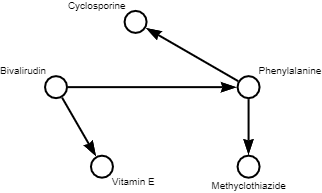
\includegraphics[width=0.5\linewidth]{chapters/background/figures/ddi.png} 
    \caption{Homogeneous Drug-Drug Interaction Graph.}
    \label{fig:sample_ddi}
\end{figure}

Graph is heterogeneous if the set of nodes can be partitioned into disjoint sets $V = V_{1} \cup V_{2} \cup ... \cup V_{k} $ where $V_{i} \cap V_{j} = \emptyset , \forall i \neq j$ \cite{sun2013mining}. For instance, drug-disease network is a heterogeneous graph consisting of two types of nodes as drugs and diseases, and two types of edges representing the \textit{treatment} relation that occurs only between drug nodes and disease nodes, and similarly \textit{polypharmacy side effect} that occurs only between two drug nodes. Figure \ref{fig:sample_ddi} shows a heterogeneous drug-disease association graph with 4 drugs, three disease, and two types of edges. For instance, the risk or severity of neutropenia can be increased when Methyclothiazide is combined with Phenylalanine \cite{ruiz2022primary}. 

\begin{figure}
    \centering
        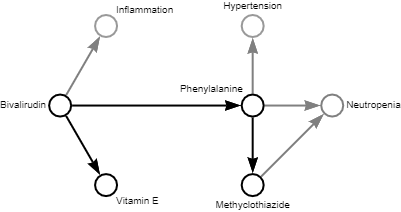
\includegraphics[width=0.65\linewidth]{chapters/background/figures/dda.png} 
    \caption{Heterogeneous Drug-Disease Association Graph.}
    \label{fig:sample_dda}
\end{figure}


\section{Graph Representation Learning}
The rapid development of molecular biology, bioinformatics, and cheminformatics and the increase in the number of available data have led the modeling the biological components as nodes and the interactions between nodes as edges of graphs. In the case of the drug discovery and disease treatment, it is crucial to examine the interactions between drug-drug, drug-disease, drug-protein, and protein-disease \cite{daminelli2012drug, davis2009comparative}. These interactions can be formed as heterogeneous graphs and used in knowledge extraction. Traditional machine learning algorithms use the data represented in Euclidean domain such as 1D sequences of proteins, 2D biomedical image, or 3D protein structure. However, graphs form a non-Euclidean domain and create a challenge due to its complex topological structure, diverse node connections, and arbitrary neighbor size. To address these challenges, graph representation learning is employed. Graph representation learning or graph embedding learns the low-dimensional representations of node or edges that can be used in downstream graph analytics or machine learning tasks such as node classification, and link prediction.

We use graph-based distributional representation learning method to represent the molecules. In general, this set of methods represents data that cannot be expressed in Euclidean space as a graph, and it aims to learn distributed vectors that reflect the semantic connections in the graph for nodes, edges or underlines in this graph \cite{wu2019comprehensive}. One of the most important advantages of this approach is that it can express the relationships between different types of nodes. Using the compiled data (See details in Chapter \ref{chapter:dataset_preparation}) we model protein, ligand, disease and side effect information and the extracted language-based information as different node types in a graph. The relationship between each node corresponds to different relationships such as protein-drug interaction and protein-protein interaction in our graph. By using the heterogeneous graph structure that we have obtained in this way, we learn the graph-based representation vectors for proteins and chemicals. In this heterogeneous graph, when distributional representations for chemicals and proteins are learned, the relationships of nodes with different concepts such as disease and side effects are also included in the representations. In this way, the output of the received vectors becomes richer in terms of information. 

To learn the distributional representation vectors we use MetaPath2Vec \cite{dong2017metapath2vec, pal2016deep}, which is a framework to learn representations of heterogeneous graphs. It is a neural network model that is designed to capture the rich semantics embedded in heterogeneous graphs by exploiting different types of relationships and meta-paths among nodes. To generate meaningful representations, it considers different semantics of relations, i.e., different meta-paths which are the sequence of node/edge types that denote relationships between node pairs.

MetaPath2Vec formalizes the representation learning problem in heterogeneous networks by leveraging the definitions in \cite{dong2017metapath2vec, sun2013pathselclus} as follows:

A heterogeneous network is a graph $G = (V, E, T)$ in which node $v$ is associated with edge $e$ with mapping functions $\phi(v) : V \to T_{V}$ and $\varphi(e) : E \to T_{E}$, respectively. The aim of heterogeneous network representation learning is to learn the d-dimensional representation $X \in R^{|V|\times d}, d \ll |V|$ , given a heterogeneous network $G$, that is able to capture the topological and semantic relations among them. Therefore, the resulting representation is low-dimensional matrix $X$, with the $v^{th}$  row corresponding to the representation of node $v$. Regardless of the node types in $V$, representations of each node are mapped into the same latent space. 

The word2vec model is proposed to learn the distributed representations of words within a corpus \cite{mikolov2013efficient, mikolov2013distributed}. Thereafter, DeepWalk \cite{perozzi2014deepwalk} and node2vec \cite{grover2016node2vec} models proposed, aiming to map the word-context concept of word2vec model into a network. DeepWalk and node2vec models use random walks to map the word-context concept and utilize the skip-gram model to learn the node representation in a homogeneous network. Their objective is to maximize the network probability \cite{mikolov2013distributed, perozzi2014deepwalk, grover2016node2vec}, that is:
\begin{equation}
    arg \max_{\theta} \prod_{v \in V}^{} \prod_{c \in N(V)}^{} p(c|v;\theta)
\end{equation}

where $N(v)$ denotes the node $v$'s neighborhood, in which $v$'s one-hop neighbors, and $p(c|v;\theta)$ defines the conditional probability of a context node $c$ given node $v$.

In the same way, metapath2vec introduces the heterogeneous skip-gram model for heterogeneous networks to model the heterogeneous neighborhood of a node. Therefore, metapath2vec aims to maximize the probability of having the heterogeneous context $N_{t}(v), t \in T_{V}$ given a node $v$:

\begin{equation}
    arg \max_{\theta} \sum_{v \in V}^{} \sum_{t \in T_{V} }^{} \sum_{c_{t} \in N_{t}(V)}^{} p(c_{t}|v;\theta)
\label{eq:context}
\end{equation}

where $N_{t}(v)$ denotes the node $v$'s neighborhood with the $t^{th}$ type of nodes. The $p(c_{t}|v;\theta)$ is a softmax function \cite{bengio2013representation, mikolov2013distributed}, that is:

\begin{equation}
    p(c_{t}|v;\theta) = \frac{e^{X_{c_{t}}}.X_{v}}{\sum_{u \in V}^{} e^{X_{u}}.X_{v}}
\label{eq:softmax}
\end{equation}

where $X_{v}$ is the $v^{th}$ row of $X$, corresponding to the embedding vector for node $v$. Mikolov \textit{et al.} also introduce negative sampling \cite{mikolov2013distributed} for optimization. With negative sampling, a small set of words are sampled from the corpus to construct the softmax. Same technique is also applied for metapath2vec, and Equation \ref{eq:context} is updated as follows:

\begin{equation}
    log\sigma(X_{c_{t}}.X_{v}) + \sum_{m=1}^{M} \mathbb{E}_{u^{m}\sim P(u)}[log\sigma(-X_{u^{m}}.X_{v})]
\end{equation}

where $M$ is the negative sample size, $\sigma (x) = \frac{1}{1+e^{-x}}$ and $P(u)$ is the pre-defined distribution in which node $u^{m}$ is drew from $M$ times.

In order to transform heterogeneous network structures into metapath2vec's skip-gram, that design a meta-path-based random walks, and generate paths. A meta-path schema is a path, denoted as $V_{1} \xrightarrow[]{R_{1}} V_{2} \xrightarrow[]{R_{2}}\cdots V_{t} \xrightarrow[]{R_{t}} V_{t+1} \cdots \xrightarrow[]{R_{l-1}} V_{l}$, where $R = R_{1} \circ R_{2} \circ \cdots \circ R_{l-1}$ defines the composite relations between node types $V_{1}$ and $V_{l}$ \cite{sun2012mining}.

As shown above, metapath2vec uses random walks guided by meta-paths to generate heterogeneous node sequences that are rich in semantics and structural information, then it designs a heterogeneous skip-gram model to preserve the node $v$'s proximity to its neighborhood nodes. It uses Equation \ref{eq:softmax} to calculate the similarity a node and its neighbors.

Based on metapath2vec, several variants have been proposed. For instance, BHIN2vec \cite{lee2019bhin2vec} proposes an extension to the skip-gram technique in order to balance the influence different relation types on node embeddings. HHNE \cite{wang2019hyperbolic} performs random walks in hyperbolic spaces. Another method, Hin2vec \cite{fu2017hin2vec}, combines first-order and high-order relations to capture the heterogeneity of graph and carries out multiple relation prediction tasks to jointly learn the node embeddings. In this thesis we employ metapath2vec since it is simpler and convenient to apply to large heterogeneous graph. Moreover, its code is open, so it is freely available to use and easy to adapt.\footnote{Code available at: https://github.com/apple2373/metapath2vec}

\section{Language-Based Representation Vector Learning}

\section{Affinity Prediction}

\section{Evaluation}
\chapter{DATASET PREPARATION}
\label{chapter:dataset_preparation}

In this thesis, we predict the affinity score of drug-target pairs by using heterogeneous networks generated with the existing information of chemicals, proteins, and enriched with additional information extracted from the text representations of these biomolecules.

We compiled several databases in order to use different data types as inputs to our models to learn the distributional representation vectors of molecules. In this chapter we conduct a literature review about the databases, up-to-date statistical data, and the usage of the information.

\section{BindingDB}
BindingDB \cite{gilson2016bindingdb} is an accessible database of drug target interactions and measured binding affinity values. With statistics as of February 2021, it can be listed as follows: It contains 41.328 entries, 8.202 protein targets each with a DOI, and 2.114.159 binding data for 928.022 small molecules. There are 2,823 protein-ligand crystal structures with BindingDB binding affinity measures for proteins with 100\% sequence identity, and 8.263 crystal structures allowing 85\% sequence identity of proteins. 2.077.458 Ki (nM), Kd (nM), IC50 (nM), EC50 (nM) values were compiled from the database within the scope of the thesis. 

To benchmark the performance of graph-based representational learning we use BDB dataset \cite{ozccelik2021chemboost} that is extracted from the BindingDB database. 24.404 binding affinities observed for all pairs of 924 ligand and 480 proteins, measured by the $pK_d$ value (log transformed kinase dissociation constant). The number of ligands with strong binding affinity values is 3428 (i.e., $pK_d \geq 7$) according to literature \cite{he2017simboost}. Figure \ref{fig:bdb} illustrates the distribution of the binding affinity values of proteins - ligand pairs in BDB dataset. 

\begin{figure}
    \centering
        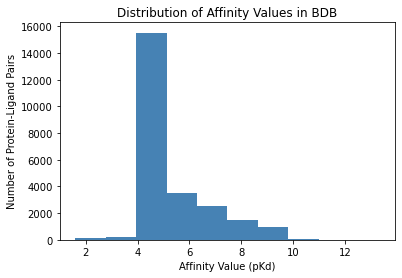
\includegraphics[width=0.5\linewidth]{chapters/datasetpreparation/figures/bdb.png} 
    \caption{Distribution of binding affinity values in BDB.}
    \label{fig:bdb}
\end{figure}

BDB dataset consists of 5 different setups for training and evaluating the model performance. To evaluate the performance of DeepDTA, we trained DeepDTA model with the knowledge derived from heterogeneous networks on five training setups of BDB dataset \cite{ozccelik2021chemboost}, and test the models in the corresponding test sets. 
\section{DrugBank}
DrugBank \cite{wishart2006drugbank, wishart2008drugbank, wishart2018drugbank} is an online database of information about drugs and drug targets. It contains information about drugs, such as chemical, pharmacological, and pharmaceutical data, and information about drug targets, such as sequence, structure, and pathways, as both bioinformatics and cheminformatics sources. Statistical information as of January 2021 is given in Table 
\ref{tab:drugbank_stats}. 14.350 drugs and 2.682.158 drug-drug interaction information from DrugBank were compiled as data within the scope of the project.

\begin{table}[]
\caption{DrugBank statistics (01.2021).}
\centering
\begin{tabular}{|l|l|}
\hline
\multicolumn{1}{|c|}{\textbf{Data}}  & \multicolumn{1}{c|}{\textbf{Number}} \\ \hline
Total Number of Small Molecule Drugs & 11.834                               \\ \hline
Total Number of Biotech Drugs        & 2.481                                \\ \hline
Total Number of Drugs                & 14.315                               \\ \hline
\end{tabular}
\label{tab:drugbank_stats}
\end{table}
\section{SIDER}

SIDER \cite{kuhn2010side, kuhn2016sider} is a database of drugs that have entered the market and their recorded adverse drug reactions extracted from public documents and prospectuses. Information such as side effect frequency, drug and side effect classification, and drug-target relationships are presented in a computer readable format. SIDER uses the Anatomical Therapeutic Chemical (ATC) Classification System, which is a drug classification system that classifies the active substances of drugs according to the organ or system they act on and their therapeutic, pharmacological and chemical properties. Side effects are coded by converting to MedDRA terminology. The current statistics of the data in the database are shown in Table \ref{tab:sider_stats}. From these data, 5,868 side effects and 139,756 drug-side effect relations were compiled within the scope of this thesis.

\begin{table}[]
\caption{SIDER Database statistics (10.2015).}
\centering
\begin{tabular}{|l|l|l|}
\hline
\textbf{Side Effects} & \textbf{Drugs} & \textbf{Drug-Side Effect Pairs} \\ \hline
5.868        & 1.430 & 139.756 \\ \hline
\end{tabular}
\label{tab:sider_stats}
\end{table}
\section{Comparative Toxicogenomics Database}
The Comparative Toxicogenomics Database \cite{davis2021comparative}, CTD, is a database that provides information on manually curated chemical–gene/protein interactions, chemical–disease and gene–disease relationships. CTD has several categories of data. These are chemicals, diseases, chemical-disease relationships, and gene-disease relationships. Statistical data as of February 2021 are given in Table \ref{tab:ctd_stats}. From these data, a total of 2.958.797 chemical-disease relationship and 28.253.189 gene-disease relationship data were compiled within the scope of the project.

\begin{table}[]
\caption{CTD statistics (02.2021).}
\centering
\begin{tabular}{|l|l|}
\hline
\multicolumn{1}{|c|}{\textbf{Data}} & \multicolumn{1}{c|}{\textbf{Number}} \\ \hline
Chemicals                  & 16.572                      \\ \hline
Diseases                   & 7.246                       \\ \hline
Chemical-Disease Relation  & 2.958.797                   \\ \hline
Gene-Disease Relation      & 28.253.189                  \\ \hline
\end{tabular}
\label{tab:ctd_stats}
\end{table}
\section{PubChem}
PubChem is an open chemistry database that contains small molecules, nucleotides, carbohydrates, lipids, peptides, and chemically-modified macromolecules, as well as information on chemical structures, identifiers, chemical and physical properties, biological activities, patents, health, safety, and toxicity data about them. Current statistics in the database are given in Table \ref{tab:pubchem_stats}.

\begin{table}[]
\caption{PubChem statistics (02.2021)}
\centering
\begin{tabular}{|l|l|}
\hline
\multicolumn{1}{|c|}{\textbf{Data}} & \multicolumn{1}{c|}{\textbf{Number}} \\ \hline
Compounds                           & 109.487.163                          \\ \hline
Substances                          & 270.034.522                          \\ \hline
Proteins                            & 96.280                               \\ \hline
Genes                               & 89.655                               \\ \hline
\end{tabular}
\label{tab:pubchem_stats}
\end{table}

 

\section{Universal Protein Resource}
The Universal Protein Source (UniProt) \cite{uniprot2021uniprot}, is an important resource for accessible protein information including protein sequence and functional information. As of June 2021, the total number of entries is 565.254  according to current statistics. 

\section{STRING}
Search Tool for the Retrieval of Interacting Genes/Proteins, STRING \cite{szklarczyk2021string}, is a biological database of known and predicted protein-protein interactions. The interactions include direct (physical) and indirect (functional) associations; they stem from computational prediction, from knowledge transfer between organisms, and from interactions aggregated from other (primary) databases.

The STRING database compiles information from several sources such as computational prediction methods, public text collections, laboratory experiments, and other databases. According to the statistics provided as of August 2021, the STRING database contains 67.592.464 proteins and 296.567.750 interactions at highest security (score $>=$ 0.900),  834.790.438 interactions with high security or better (score $>=$ 0.700), medium security or better 3.112.520.562 interactions (score $>=$ 0.400), and a total of 20,052,394,041 interactions.
\section{ChEMBL}
ChEMBL \cite{davies2015chembl, gaulton2017chembl} is a manually curated chemical database of molecules with drug-like properties and biological activity which is maintained by the European Molecular Biology Laboratory (EMBL). The ChEMBL database contains bioactivity data of pharmaceutical active ingredients which are reported with Ki, Kd, IC50 and EC50 values. ChEMBL examines how small molecules interact with target proteins, and how these compounds affect cells and whole organisms. Moreover, ChEMBL includes information about the 2D structure, calculated molecular properties, and the ADMET properties, which are assessment of in vivo absorption, distribution, metabolism, excretion and toxicity of small molecules. According to the statistics as of May, 2020, there are 1.941.412 chemicals in the ChEMBL database.
\section{Data Assembling}

Our idea was to represent chemicals and proteins better. Therefore, we compiled chemical and proteins related data from several online databases. And the challenging task was to assemble these compiled large data. For that purpose we analyze the available information in above mentioned databases and and map related information using common data. 

\subsection{Chemical Related Information}
DrugBank, PubChem, and ChEMBL databases are the main resources of chemicals and we mainly focus on them. As an initial step we compile 14.350 drugs from DrugBank and retrieve their DrugBank IDs and InChi (International Chemical Identifier) Keys. Using InChI keys, we map the data in DrugBank to PubChem and ChEMBL databases and able to get the information about 10.935 distinct drugs. With 10.935 drugs, we extract 2.196.820 drug-drug relation information from DrugBank database. Using the PubChem CID (Compound ID number) information available at PubChem database, we map the PubChem to SIDER and CTD databases. From SIDER database, we extract 5452 distinct side effects and 115.871 drug-side effect association information for 1003 drugs. From CTD database, we extract 7086 distinct diseases and 995.654 drug-disease association information for 3387 drugs. Finally, using the InChI keys, we map DrugBank to ChEMBL and compile SMILES (Simplified molecular-input line-entry system) representations of 10.935 drugs. 

\subsection{Protein Related Information}
UniProt and STRING databases are main resources used in this thesis. We compile 505.250 proteins from the UniProt database and more specifically we compile 202.160 proteins belonging to the Homo sapiens, as well as their amino acid sequences. Using the UniProt ID from UniProt database, we map 18.876 proteins to STRING database, and extract 183.746 protein-protein interaction information. Finally, using the UniProt ID and Entrez Gene ID we map UniProt database to CTD and extract 32.495 protein-disease association information for 32.169 proteins and 126 distinct diseases.
%assembling a het database

\chapter{EMPOWERING HETEROGENEOUS DATA WITH BIOMOLECULAR LANGUAGE}
\chapter{RESULTS}

\section{Evaluation}
Representation vectors for chemicals and proteins obtained using the aforementioned models and graphs, and then these vectors evaluated in the drug-target affinity task with the DeepDTA model using the BDB dataset. The DeepDTA model represents proteins using amino acid sequences and chemicals using characters of the SMILES notations. In this study, the DeepDTA model has been updated, as shown in Figure 3.3, to take as input the representation vectors containing additional information in the generated graphs. The performance of the model is measured by the Concordance Index (CI),  Mean Squared Error (MSE), Root Mean Squared Error (RMSE), and $R2$ metrics. 

% explain metrics with formula

\section{Experimental Setup}

As the training and test folds we use the same setup used in DeepDTA \cite{ozturk2018deepdta}. We train each model 5 times with the training set folds, then measure the performance on each test set, and report the average results on BDB. BDB dataset contains 5 different training sets and corresponding 4 different test sets as warm, cold ligand, cold protein and cold. The cold test sets contain data that was not used during the training of the model. We compute CI, MSE, RMSE, and $R^2$ scores of each model and report with the standard deviation.


\section{Model Comparisons}

\paragraph{Homogeneous ligand representation}
First, we generate homogeneous graphs with only one node and edge type, then test WideDeepDTA performance for the ligand representation.

\begin{itemize}
    \item \textbf{Model (1)}: A DDI (Drug-Drug Interaction) graph is created, the nodes of which are formed by all drugs (D) and the edges by interactions (D-D) between these drugs.   
    \item \textbf{Model (2)}: A DDI graph is created similar to Model (1), this time with the knowledge of initial embeddings of ChemBERTa model.
    \item \textbf{Model (3)}: A DDS (Drug-Drug Similarity) graph is created, the nodes of which are formed by all drugs (D) and the edges by Jaccard similarity between these drugs. 
    \item \textbf{Model (4)}: A DDS graph is created similar to Model (3), this time with the knowledge of initial embeddings of ChemBERTa model.
\end{itemize}

We first test the impact of ligand representation using homogeneous graphs by creating two different models with two different versions. Model (1) represents each drug with a 32-dimensional vector in which they are initialized as samples
from a uniform distribution over $[0, 1)$ and trained by metapath2vec model on DDI relation, and Model (2) represents each drug with the same dimensional size vector, however metapath2vec model's embeddings are initialized as ChemBERTa embeddings of corresponding ligands. (For the detailed results please refer to the Appendix \ref{app:homogeneous_ligand} and see Table \ref{tab:ddi_ci_r2} and Table \ref{tab:ddi_mse_rmse}.) On the other hand, Model (3) and Model (4) are trained on DDS relation with the same setup. (For the detailed results please refer to the Appendix \ref{app:homogeneous_ligand} and see Table \ref{tab:dds_ci_r2} and Table \ref{tab:dds_mse_rmse}.)

The results regarding the comparison of these four models are shown in Table \ref{tab:ddi_vs_dds_warm}, Table \ref{tab:ddi_vs_dds_cold_prot}, Table \ref{tab:ddi_vs_dds_cold_ligand}, and Table \ref{tab:ddi_vs_dds_cold_both}. Considering the results shown in Table \ref{tab:ddi_vs_dds_warm};
\begin{itemize}
    \item DDI models and DDS models perform similarly on the warm test set of BDB, \textit{i.e.}, their trends are the same for the same performance metrics. For instance, value of $R^2$ for models with PLMs is higher than the randomly initialized models, likewise MSE and RMSE values are lower for DDI and DDS models for the same case.
    \item Using PLM for drugs actually works since it increases the performance for three out of four metrics for both of the DDI and DDS models.
    \item As a result, we claim that, one can employ the similarity measures between two drugs when the interaction information is not available for these two drugs while using empowered homogeneous graphs on warm test set of BDB.
\end{itemize}

\begin{table}[H]
\centering
\caption{Scores of DDI and DDS models on \textbf{warm} test set of BDB.}
\label{tab:ddi_ci_r2}
\begin{tabular}{|l|l|c|l|l|} 
\hline
Model & \multicolumn{1}{c|}{CI} & $R^2$ & \multicolumn{1}{c|}{MSE} & \multicolumn{1}{c|}{RMSE} \\ 
\hline
DeepDTA & 0.888 (0.009) & 0.781 (0.028) & 0.288 (0.021) & 0.536 (0.012) \\ 
\hline
Model (1) & \textbf{0.896 (0.009)} & 0.777 (0.026) & 0.295 (0.036) & 0.542 (0.033) \\ 
\hline
Model (2) & 0.890 (0.014) & 0.782 (0.017) & 0.287 (0.014) & 0.535 (0.014) \\ 
\hline
Model (3) & 0.893 (0.005) & 0.787 (0.020) & 0.280 (0.017) & 0.529 (0.017) \\ 
\hline
Model (4) & 0.890 (0.006) & \textbf{0.789 (0.008)} & \textbf{0.278 (0.011)} & \textbf{0.527 (0.010)} \\
\hline
\end{tabular}
\label{tab:ddi_vs_dds_warm}
\end{table}


As stated in the work of DeepDTA, CNN's ability to represent protein sequences is very low \cite{ozturk2018deepdta}. We initialized all the protein embeddings with zeros, since we do not train our models with any kinds of protein-related information. Considering the results shown in Table \ref{tab:ddi_vs_dds_cold_prot}, even initializing with zeros increases the performance for the DDI model. 


\begin{table}[H]
\centering
\caption{Scores of DDI and DDS models on \textbf{cold protein} test set of BDB.}
\label{tab:ddi_ci_r2}
\begin{tabular}{|l|l|c|l|l|} 
\hline
Model & \multicolumn{1}{c|}{CI} & $R^2$ & \multicolumn{1}{c|}{MSE} & \multicolumn{1}{c|}{RMSE} \\ 
\hline
DeepDTA & 0.759 (0.006) & 0.315 (0.049) & 1.085 (0.146) & 1.040 (0.146) \\ 
\hline
Model (1) & \textbf{0.779 (0.030)} & \textbf{0.375 (0.104)} & \textbf{0.992 (0.207)} & \textbf{0.991 (0.101)} \\ 
\hline
Model (2) & 0.768 (0.009) & 0.327 (0.072) & 1.064 (0.154) & 1.029 (0.077) \\ 
\hline
Model (3) & 0.775 (0.018) & 0.340 (0.082) & 1.045 (0.174) & 1.019 (0.086) \\ 
\hline
Model (4) & 0.774 (0.015) & 0.327 (0.075) & 1.065 (0.162) & 1.029 (0.079) \\
\hline
\end{tabular}
\label{tab:ddi_vs_dds_cold_prot}
\end{table}

Taking into consideration the results shown in Table \ref{tab:ddi_vs_dds_cold_ligand} and Table \ref{tab:ddi_vs_dds_cold_both}, adding drug-related information using the homogeneous graph or empowered homogeneous graph did not improve the performance for the cold ligand and cold both test cases. However, results for cold both test set slightly better then the cold ligand test set due to the performance improvement of cold proteins. 

<<<<<<< Updated upstream
=======
<<<<<<< HEAD
\begin{table}
\centering
\caption{Scores of DDI and DDS models on cold ligand test set of BDB.}
\vspace{0.25em}
=======
>>>>>>> Stashed changes
\begin{table}[H]
\centering
\caption{Scores of DDI and DDS models on \textbf{cold ligand} test set of BDB.}
\label{tab:ddi_ci_r2}
<<<<<<< Updated upstream
=======
>>>>>>> d09ebba9e602d1522ef9361417dc21d129009597
>>>>>>> Stashed changes
\begin{tabular}{|l|l|c|l|l|} 
\hline
Model & \multicolumn{1}{c|}{CI} & $R^2$ & \multicolumn{1}{c|}{MSE} & \multicolumn{1}{c|}{RMSE} \\ 
\hline
DeepDTA & \textbf{0.687 (0.096)} & \textbf{0.039 (0.243)} & \textbf{1.448 (0.939)} & \textbf{1.152 (0.348)} \\ 
\hline
Model (1) & 0.664 (0.057) & -0.053 (0.210) & 1.472 (0.650) & 1.187 (0.249) \\ 
\hline
Model (2) & 0.640 (0.066) & -0.125 (0.180) & 1.548 (0.602) & 1.225 (0.220) \\ 
\hline
Model (3) & 0.651 (0.085) & -0.139 (0.132) & 1.603 (0.645) & 1.242 (0.246) \\ 
\hline
Model (4) & 0.666 (0.064) & -0.102 (0.330) & 1.502 (0.615) & 1.202 (0.239) \\
\hline
\end{tabular}
\label{tab:ddi_vs_dds_cold_ligand}
\end{table}
<<<<<<< Updated upstream
=======
<<<<<<< HEAD
\begin{table}
\centering
\caption{Scores of DDI and DDS models on cold both test set of BDB.}
\vspace{0.25em}
=======
>>>>>>> Stashed changes
\begin{table}[H]
\centering
\caption{Scores of DDI and DDS models on \textbf{cold both} test set of BDB.}
\label{tab:ddi_ci_r2}
<<<<<<< Updated upstream
=======
>>>>>>> d09ebba9e602d1522ef9361417dc21d129009597
>>>>>>> Stashed changes
\begin{tabular}{|l|l|c|l|l|} 
\hline
Model & \multicolumn{1}{c|}{CI} & $R^2$ & \multicolumn{1}{c|}{MSE} & \multicolumn{1}{c|}{RMSE} \\ 
\hline
DeepDTA & \textbf{0.554 (0.047)} & \textbf{-0.154 (0.164)} & \textbf{2.007 (1.223)} & \textbf{1.356 (0.410)} \\ 
\hline
Model (1) & 0.554 (0.044) & -0.287 (0.184) & 2.013 (0.767) & 1.395 (0.260) \\ 
\hline
Model (2) & 0.495 (0.037) & -0.496 (0.211) & 2.348 (0.978) & 1.504 (0.294) \\ 
\hline
Model (3) & 0.519 (0.036) & -0.390 (0.235) & 2.278 (1.069) & 1.467 (0.356) \\ 
\hline
Model (4) & 0.536 (0.068) & -0.274 (0.269) & 2.021 (0.950) & 1.388 (0.308) \\
\hline
\end{tabular}
\label{tab:ddi_vs_dds_cold_both}
\end{table}

\paragraph{Homogeneous protein representation}
Second, we generate homogeneous graphs with only one node and edge type, then test WideDeepDTA performance for the protein representation.

\begin{itemize}
    \item \textbf{Model (5)}: A PPI (Protein-Protein Interaction) graph is created, the nodes of which are formed by all proteins (P) and the edges by interactions (P-P) between these proteins.   
    \item \textbf{Model (6)}: A PPI graph is created similar to Model (3), this time with the knowledge of initial embeddings of ProtBERT model.
    \item \textbf{Model (7)}: A PPS (Protein-Protein Similarity) graph is created, the nodes of which are formed by all proteins belonging to the human species (P) and the edges formed by the Jaccard similarities (P-P) between the amino acid sequences of these proteins. While calculating the similarities we tokenized each amino acid sequence using the glossary generated by BPE. Then we calculate the Paired Jaccard similarities of protein tokens. Considering the dataset, a threshold value is determined to cover at least 11\% of the data. Accordingly, protein pairs with similarity values greater than 9 determined to be similar to each other. 
    \item \textbf{Model (8)}: A PPS graph is created similar to Model (7), this time with the knowledge of initial embeddings of ProtBERT model.
\end{itemize}

First, we test the impact of protein representation using homogeneous graphs by creating two different models with two different versions. Model (5) represents each protein with a 32-dimensional vector in which they are initialized as samples from a uniform distribution over $[0, 1)$ and trained by metapath2vec model on PPI relation, and Model (6) represents each drug with the same dimensional size vector, however metapath2vec model's embeddings are initialized as ProtBERT embeddings of corresponding proteins. (For the detailed results please refer to the Appendix \ref{app:homogeneous_protein} and see Table \ref{tab:ppi_ci_r2} and Table \ref{tab:ppi_mse_rmse}.) On the other hand, Model (7) and Model (8) are trained on PPS relation with the same setup. (For the detailed results please refer to the Appendix \ref{app:homogeneous_protein} and see Table \ref{tab:pps_ci_r2} and Table \ref{tab:ppse_mse_rmse}.)

The results regarding the comparison of these four models are shown in Table \ref{tab:ppi_vs_pps_warm}, Table \ref{tab:ppi_vs_pps_cold_protein}, Table  \ref{tab:ppi_vs_pps_cold_ligand}, and Table \ref{tab:ppi_vs_pps_cold_both}. Considering the results shown in Table \ref{tab:ppi_vs_pps_warm};
\begin{itemize}
    \item Empowered graphs generated by PPS relation adds more information to the representation of proteins compared to the empowered graphs generated by PPI relation on warm test set. 
    \item In the case of PPI models, model with empowered graph performs better than the normal graphs in all metrics, except CI. However, both of them perform worse than the DeepDTA model on warm test set.
\end{itemize}

Considering the results shown in Table \ref{tab:ppi_vs_pps_cold_protein};
\begin{itemize}
    \item Empowered graphs generated by PPS relation adds more information to the representation of proteins compared to the empowered graphs generated by PPI relation on warm test set. 
    \item In the case of PPI models, model with empowered graph performs better than the normal graphs in all metrics, except CI. However, both of them perform worse than the DeepDTA model on warm test set.
\end{itemize}

<<<<<<< Updated upstream
=======
<<<<<<< HEAD
\begin{table}
\centering
\caption{Scores of PPI and PPS models on warm test set of BDB.}
\vspace{0.25em}
=======
>>>>>>> Stashed changes
\begin{table}[H]
\centering
\caption{Scores of PPI and PPS models on \textbf{warm} test set of BDB.}
\label{tab:ddi_ci_r2}
<<<<<<< Updated upstream
=======
>>>>>>> d09ebba9e602d1522ef9361417dc21d129009597
>>>>>>> Stashed changes
\begin{tabular}{|l|l|c|l|l|} 
\hline
Model & \multicolumn{1}{c|}{CI} & $R^2$ & \multicolumn{1}{c|}{MSE} & \multicolumn{1}{c|}{RMSE} \\ 
\hline
DeepDTA & 0.888 (0.009) & 0.781 (0.028) & 0.288 (0.021) & 0.536 (0.012) \\ 
\hline
Model (5) & 0.888 (0.009) & 0.773 (0.025) & 0.299 (0.020) & 0.546 (0.018) \\ 
\hline
Model (6) & 0.888 (0.009) & 0.777 (0.012) & 0.295 (0.017) & 0.543 (0.015) \\ 
\hline
Model (7) & \textbf{0.893 (0.006)} & 0.775 (0.018) & 0.296 (0.018) & 0.544 (0.016) \\ 
\hline
Model (8) & 0.892 (0.008) & \textbf{0.785 (0.019)} & \textbf{0.283 (0.015)} & \textbf{0.532 (0.015)} \\
\hline
\end{tabular}
\label{tab:ppi_vs_pps_warm}
\end{table}

\paragraph{Heterogeneous representations}
Third, we generate heterogeneous graphs with several node and edge types, then test WideDeepDTA performance for the ligand representation.

\begin{itemize}
    \item \textbf{Model (9)} A DDiA (Drug-Disease Association) graph is created, the nodes of which are formed by all drugs (D), and diseases (Di) and the edges by association (D-Di) between these drugs and diseases.  
    \item \textbf{Model (10)} A DDiA graph is created similar to Model (9), this time with the knowledge of initial embeddings of ChemBERTa and BioBert models for SMILES sequences and disease names.
    \item \textbf{Model (15)} A DSA (Drug-Side Effect Association) graph is created, the nodes of which are formed by all drugs (D), and side effects (S) and the edges by association (D-S) between these drugs and side effects.  
    \item \textbf{Model (16)} A DSA graph is created similar to Model (15), this time with the knowledge of initial embeddings of ChemBERTa and BioBert models for SMILES sequences and side effect names.
    \item \textbf{Model (17)} A DDI-DSA (Drug-Drug Interaction \& Drug-Side Effect Association) graph is created, the nodes of which are formed by all drugs (D), and side effects (S) and the edges by association (D-D and D-S) between these drugs and side effects.  
    \item \textbf{Model (18)} A DDI-DSA graph is created similar to Model (17), this time with the knowledge of initial embeddings of ChemBERTa and BioBert models for SMILES sequences and side effect names.
\end{itemize}

% \usepackage{multirow}


\begin{table}
\centering
\caption{CI and R$^2$ scores of DDiA models on test sets of BDB.}
\label{tab:ddi_ci_r2}
\begin{tabular}{|l|l|c|c|} 
\hline
\begin{tabular}[c]{@{}l@{}}\\\textbf{Model}\end{tabular} & \textbf{Test~Set} & \textbf{CI} & \textbf{R\textsuperscript{2}} \\ 
\hline
DeepDTA & \multirow{3}{*}{Warm} & 0.888 (0.009) & 0.781 (0.028) \\ 
\cline{1-1}\cline{3-4}
Model (9) &  & 0.895 (0.013) & \textbf{0.786 (0.023)} \\ 
\cline{1-1}\cline{3-4}
Model (10) &  & \textbf{0.896 (0.006)} & 0.784 (0.019) \\ 
\hline
DeepDTA & \multirow{3}{*}{\begin{tabular}[c]{@{}l@{}}Cold\\Ligand\end{tabular}} & 0.687 (0.096) & 0.039 (0.243) \\ 
\cline{1-1}\cline{3-4}
Model (9) &  & 0.690 (0.050) & -0.025 (0.202) \\ 
\cline{1-1}\cline{3-4}
Model (10) &  & \textbf{0.695 (0.056)} & \textbf{0.066 (0.122)} \\ 
\hline
DeepDTA & \multirow{3}{*}{\begin{tabular}[c]{@{}l@{}}Cold\\Protein\end{tabular}} & 0.759 (0.006) & 0.315 (0.049) \\ 
\cline{1-1}\cline{3-4}
Model (9) &  & \textbf{0.784 (0.010)} & \textbf{0.349 (0.072)} \\ 
\cline{1-1}\cline{3-4}
Model (10) &  & 0.779 (0.014) & 0.333 (0.089) \\ 
\hline
DeepDTA & \multirow{3}{*}{Cold} & 0.554 (0.047) & \textbf{-0.154 (0.164)} \\ 
\cline{1-1}\cline{3-4}
Model (9) &  & \textbf{0.567 (0.047)} & -0.187 (0.177) \\ 
\cline{1-1}\cline{3-4}
Model (10) &  & 0.564 (0.031) & -0.201 (0.095) \\
\hline
\end{tabular}
\label{tab:ddia_ci_r2}
\end{table}
% \usepackage{multirow}


\begin{table}
\centering
\caption{MSE and RMSE scores of DDiA models on test sets of BDB.}
\label{tab:ddi_ci_r2}
\begin{tabular}{|l|l|c|c|} 
\hline
\begin{tabular}[c]{@{}l@{}}\\\textbf{Model}\end{tabular} & \textbf{Test~Set} & \textbf{MSE} & \textbf{RMSE} \\ 
\hline
DeepDTA & \multirow{3}{*}{Warm} & 0.288 (0.021) & 0.536 (0.012) \\ 
\cline{1-1}\cline{3-4}
Model (9) &  & \textbf{0.282 (0.023)} & \textbf{0.530 (0.022)} \\ 
\cline{1-1}\cline{3-4}
Model (10) &  & 0.284 (0.015) & 0.533 (0.014) \\ 
\hline
DeepDTA & \multirow{3}{*}{\begin{tabular}[c]{@{}l@{}}Cold\\Ligand\end{tabular}} & 1.448 (0.939) & 1.152 (0.348) \\ 
\cline{1-1}\cline{3-4}
Model (9) &  & 1.381 (0.443) & 1.162 (0.177) \\ 
\cline{1-1}\cline{3-4}
Model (10) &  & \textbf{1.294 (0.476)} & \textbf{1.120 (0.202)} \\ 
\hline
DeepDTA & \multirow{3}{*}{\begin{tabular}[c]{@{}l@{}}Cold\\Protein\end{tabular}} & 1.085 (0.146) & 1.040 (0.146) \\ 
\cline{1-1}\cline{3-4}
Model (9) &  & \textbf{1.032 (0.161)} & \textbf{1.013 (0.080)} \\ 
\cline{1-1}\cline{3-4}
Model (10) &  & 1.057 (0.191) & 1.024 (0.093) \\ 
\hline
DeepDTA & \multirow{3}{*}{Cold} & 2.007 (1.223) & 1.356 (0.410) \\ 
\cline{1-1}\cline{3-4}
Model (9) &  & \textbf{1.873 (0.792)} & \textbf{1.341 (0.271)} \\ 
\cline{1-1}\cline{3-4}
Model (10) &  & 1.939 (0.854) & 1.360 (0.298) \\
\hline
\end{tabular}
\label{tab:ddia_mse_rmse}
\end{table}
% \usepackage{multirow}


\begin{table}
\centering
\caption{CI and R$^2$ scores of DSA models on test sets of BDB.}
\label{tab:ddi_ci_r2}
\begin{tabular}{|l|l|c|c|} 
\hline
\begin{tabular}[c]{@{}l@{}}\\\\\textbf{Model}\end{tabular} & \textbf{Test~Set} & \textbf{CI} & \textbf{R\textsuperscript{2}} \\ 
\hline
DeepDTA & \multirow{3}{*}{Warm} & 0.888 (0.009) & 0.781 (0.028) \\ 
\cline{1-1}\cline{3-4}
Model (15) &  & \textbf{0.898 (0.009)} & \textbf{0.791 (0.016)} \\ 
\cline{1-1}\cline{3-4}
Model (16) &  & 0.889 (0.011) & 0.776 (0.021) \\ 
\hline
DeepDTA & \multirow{3}{*}{\begin{tabular}[c]{@{}l@{}}Cold\\Ligand\end{tabular}} & \textbf{0.687 (0.096)} & \textbf{0.039~(0.243)} \\ 
\cline{1-1}\cline{3-4}
Model (15) &  & 0.683 (0.040) & -0.074 (0.265) \\ 
\cline{1-1}\cline{3-4}
Model (16) &  & 0.664 (0.068) & -0.196 (0.196) \\ 
\hline
DeepDTA & \multirow{3}{*}{\begin{tabular}[c]{@{}l@{}}Cold\\Protein\end{tabular}} & 0.759 (0.006) & 0.315 (0.049) \\ 
\cline{1-1}\cline{3-4}
Model (15) &  & \textbf{0.774 (0.015)} & \textbf{0.358 (0.059)} \\ 
\cline{1-1}\cline{3-4}
Model (16) &  & 0.766 (0.022) & 0.323 (0.097) \\ 
\hline
DeepDTA & \multirow{3}{*}{Cold} & 0.554 (0.047) & \textbf{-0.154 (0.164)} \\ 
\cline{1-1}\cline{3-4}
Model (15) &  & 0.561 (0.045) & -0.278 (0.293) \\ 
\cline{1-1}\cline{3-4}
Model (16) &  & \textbf{0.580 (0.052)} & -0.445 (0.284) \\
\hline
\end{tabular}
\label{tab:dsa_ci_r2}
\end{table}
% \usepackage{multirow}


\begin{table}
\centering
\caption{MSE and RMSE scores of DSA models on test sets of BDB.}
\label{tab:ddi_ci_r2}
\begin{tabular}{|l|l|c|c|} 
\hline
\begin{tabular}[c]{@{}l@{}}\\\\\textbf{Model}\end{tabular} & \textbf{Test~Set} & \textbf{CI} & \textbf{R\textsuperscript{2}} \\ 
\hline
DeepDTA & \multirow{3}{*}{Warm} & 0.288 (0.021) & 0.536 (0.012) \\ 
\cline{1-1}\cline{3-4}
Model (15) &  & \textbf{0.275 (0.022)} & \textbf{0.524 (0.021)} \\ 
\cline{1-1}\cline{3-4}
Model (16) &  & 0.295 (0.021) & 0.543 (0.019) \\ 
\hline
DeepDTA & \multirow{3}{*}{\begin{tabular}[c]{@{}l@{}}Cold\\Ligand\end{tabular}} & 1.448 (0.939) & \textbf{1.152 (0.348)} \\ 
\cline{1-1}\cline{3-4}
Model (15) &  & \textbf{1.443 (0.461)} & 1.186 (0.190) \\ 
\cline{1-1}\cline{3-4}
Model (16) &  & 1.621 (0.555) & 1.258 (0.199) \\ 
\hline
DeepDTA & \multirow{3}{*}{\begin{tabular}[c]{@{}l@{}}Cold\\Protein\end{tabular}} & 1.085 (0.146) & 1.040 (0.146) \\ 
\cline{1-1}\cline{3-4}
Model (15) &  & \textbf{1.015 (0.131)} & \textbf{1.005 (0.064)} \\ 
\cline{1-1}\cline{3-4}
Model (16) &  & 1.076 (0.209) & 1.032 (0.102) \\ 
\hline
DeepDTA & \multirow{3}{*}{Cold} & 2.007 (1.223) & \textbf{1.356 (0.410)} \\ 
\cline{1-1}\cline{3-4}
Model (15) &  & \textbf{1.943 (0.647)} & 1.375 (0.228) \\ 
\cline{1-1}\cline{3-4}
Model (16) &  & 2.241 (0.905) & 1.470 (0.281) \\
\hline
\end{tabular}
\label{tab:dsa_mse_rmse}
\end{table}
% \usepackage{multirow}


\begin{table}
\centering
\caption{CI and R$^2$ scores of DDI-DSA models on test sets of BDB.}
\label{tab:ddi_ci_r2}
\begin{tabular}{|l|l|c|c|} 
\hline
\begin{tabular}[c]{@{}l@{}}\\\\\textbf{Model}\end{tabular} & \textbf{Test~Set} & \textbf{CI} & \textbf{R\textsuperscript{2}} \\ 
\hline
DeepDTA & \multirow{3}{*}{Warm} & 0.888 (0.009) & 0.781 (0.028) \\ 
\cline{1-1}\cline{3-4}
Model (17) &  & 0.892 (0.013) & 0.781 (0.021) \\ 
\cline{1-1}\cline{3-4}
Model (18) &  & \textbf{0.899 (0.008)} & \textbf{0.785 (0.017)} \\ 
\hline
DeepDTA & \multirow{3}{*}{\begin{tabular}[c]{@{}l@{}}Cold\\Ligand\end{tabular}} & 0.687 (0.096) & 0.039 (0.243) \\ 
\cline{1-1}\cline{3-4}
Model (17) &  & 0.688 (0.080) & -0.034 (0.245) \\ 
\cline{1-1}\cline{3-4}
Model (18) &  & \textbf{0.711 (0.057)} & \textbf{0.217 (0.153)} \\ 
\hline
DeepDTA & \multirow{3}{*}{\begin{tabular}[c]{@{}l@{}}Cold\\Protein\end{tabular}} & 0.759 (0.006) & 0.315 (0.049) \\ 
\cline{1-1}\cline{3-4}
Model (17) &  & 0.769 (0.019) & 0.352 (0.084) \\ 
\cline{1-1}\cline{3-4}
Model (18) &  & \textbf{0.778 (0.014)} & \textbf{0.365 (0.069)} \\ 
\hline
DeepDTA & \multirow{3}{*}{Cold} & 0.554 (0.047) & -0.154 (0.164) \\ 
\cline{1-1}\cline{3-4}
Model (17) &  & 0.569 (0.041) & -0.303 (0.244) \\ 
\cline{1-1}\cline{3-4}
Model (18) &  & \textbf{0.607 (0.061)} & \textbf{-0.018 (0.108)} \\
\hline
\end{tabular}
\label{tab:ddi_dsa_ci_r2}
\end{table}
% \usepackage{multirow}


\begin{table}
\centering
\caption{MSE and RMSE scores of DDI-DSA models on test sets of BDB.}
\label{tab:ddi_ci_r2}
\begin{tabular}{|l|l|c|c|} 
\hline
\begin{tabular}[c]{@{}l@{}}\\\\\textbf{Model}\end{tabular} & \textbf{Test~Set} & \textbf{CI} & \textbf{R\textsuperscript{2}} \\ 
\hline
DeepDTA & \multirow{3}{*}{Warm} & 0.288 (0.021) & 0.536 (0.012) \\ 
\cline{1-1}\cline{3-4}
Model (17) &  & 0.289 (0.037) & 0.537 (0.034) \\ 
\cline{1-1}\cline{3-4}
Model (18) &  & \textbf{0.285 (0.026)} & \textbf{0.533 (0.025)} \\ 
\hline
DeepDTA & \multirow{3}{*}{\begin{tabular}[c]{@{}l@{}}Cold\\Ligand\end{tabular}} & 1.448 (0.939) & 1.152 (0.348) \\ 
\cline{1-1}\cline{3-4}
Model (17) &  & 1.435 (0.640) & 1.171 (0.250) \\ 
\cline{1-1}\cline{3-4}
Model (18) &  & \textbf{1.082 (0.397)} & \textbf{1.022 (0.194)} \\ 
\hline
DeepDTA & \multirow{3}{*}{\begin{tabular}[c]{@{}l@{}}Cold\\Protein\end{tabular}} & 1.085 (0.146) & 1.040 (0.146) \\ 
\cline{1-1}\cline{3-4}
Model (17) &  & 1.026 (0.177) & 1.009 (0.086) \\ 
\cline{1-1}\cline{3-4}
Model (18) &  & \textbf{1.006 (0.162)} & \textbf{1.000 (0.081)} \\ 
\hline
DeepDTA & \multirow{3}{*}{Cold} & 2.007 (1.223) & 1.356 (0.410) \\ 
\cline{1-1}\cline{3-4}
Model (17) &  & 2.071 (0.927) & 1.406 (0.306) \\ 
\cline{1-1}\cline{3-4}
Model (18) &  & \textbf{1.608 (0.617)} & \textbf{1.245 (0.241)} \\
\hline
\end{tabular}
\label{tab:ddi_dsa_mse_rmse}
\end{table}

Fourth, we generate heterogeneous graphs with several node and edge types, then test WideDeepDTA performance for the protein representation.

\begin{itemize}
    \item \textbf{Model (11)} A PDiA (Protein-Disease Association) graph is created, the nodes of which are formed by all proteins (P) and diseases (Di) and the edges by association (P-Di) between these proteins and diseases.  
    \item \textbf{Model (12)} A PDiA graph is created similar to Model (11), this time with the knowledge of initial embeddings of ProtBERT and BioBert models for protein amino acid sequences and disease names respectively. 
\end{itemize}

Finally, we generate heterogeneous graphs with several node and edge types, then test WideDeepDTA performance for the both ligand and protein representation.

\begin{itemize}
    \item \textbf{Model (13)} A DDiPA (Drug-Disease-Protein Association) graph is created, the nodes of which are formed by all drugs (D), diseases (Di), proteins (P) and the edges by association (D-Di-P) between these drugs, proteins, and diseases.  
    \item \textbf{Model (14)} A DDiPA graph is created similar to Model (13), this time with the knowledge of initial embeddings of ChemBERTa, BioBert, and ProtBERT models for SMILES sequences, protein amino acid sequences, and disease names.
\end{itemize}

% \usepackage{multirow}


\begin{table}
\centering
\caption{CI and R$^2$ scores of DDiPA models on test sets of BDB.}
<<<<<<< Updated upstream
=======
<<<<<<< HEAD
% \label{tab:ddi_ci_r2}
\vspace{0.25em}
\begin{tabular}{|l|l|c|c|} 
\hline
\begin{tabular}[c]{@{}l@{}} \textbf{Model}\end{tabular} & \textbf{Test~Set} & \textbf{CI} & \textbf{R\textsuperscript{2}} \\ 
=======
>>>>>>> Stashed changes
\label{tab:ddi_ci_r2}
\begin{tabular}{|l|l|c|c|} 
\hline
\begin{tabular}[c]{@{}l@{}}\\\\\\\textbf{Model}\end{tabular} & \textbf{Test~Set} & \textbf{CI} & \textbf{R\textsuperscript{2}} \\ 
<<<<<<< Updated upstream
=======
>>>>>>> d09ebba9e602d1522ef9361417dc21d129009597
>>>>>>> Stashed changes
\hline
DeepDTA & \multirow{3}{*}{Warm} & \textbf{0.888 (0.009)} & \textbf{0.781 (0.028)} \\ 
\cline{1-1}\cline{3-4}
Model (13) &  & 0.878 (0.009) & 0.753 (0.020) \\ 
\cline{1-1}\cline{3-4}
Model (14) &  & 0.882 (0.008) & 0.755 (0.022) \\ 
\hline
DeepDTA & \multirow{3}{*}{\begin{tabular}[c]{@{}l@{}}Cold\\Ligand\end{tabular}} & 0.687 (0.096) & \textbf{0.039 (0.243)} \\ 
\cline{1-1}\cline{3-4}
Model (13) &  & 0.664 (0.087) & -0.040 (0.097) \\ 
\cline{1-1}\cline{3-4}
Model (14) &  & \textbf{0.703 (0.033)} & 0.030 (0.082) \\ 
\hline
DeepDTA & \multirow{3}{*}{\begin{tabular}[c]{@{}l@{}}Cold\\Protein\end{tabular}} & \textbf{0.759 (0.006)} & \textbf{0.315 (0.049)} \\ 
\cline{1-1}\cline{3-4}
Model (13) &  & 0.749 (0.018) & 0.268 (0.061) \\ 
\cline{1-1}\cline{3-4}
Model (14) &  & 0.752 (0.013) & 0.282 (0.073) \\ 
\hline
DeepDTA & \multirow{3}{*}{Cold} & 0.554 (0.047) & \textbf{-0.154 (0.164)} \\ 
\cline{1-1}\cline{3-4}
Model (13) &  & 0.533 (0.063) & -0.300 (0.161) \\ 
\cline{1-1}\cline{3-4}
Model (14) &  & \textbf{0.578 (0.050)} & -0.275 (0.123) \\
\hline
\end{tabular}
\label{tab:ddipa_ci_r2}
\end{table}
% \usepackage{multirow}


<<<<<<< Updated upstream
=======
<<<<<<< HEAD
\begin{table}[h]
\centering
\caption{MSE and RMSE scores of DDiPA models on test sets of BDB.}
\vspace{0.25em}% \label{tab:ddi_ci_r2}
\begin{tabular}{|l|l|c|c|} 
\hline
\begin{tabular}[c]{@{}l@{}} \textbf{Model}\end{tabular} & \textbf{Test~Set} & \textbf{CI} & \textbf{R\textsuperscript{2}} \\ 
=======
>>>>>>> Stashed changes
\begin{table}
\centering
\caption{MSE and RMSE scores of DDiPA models on test sets of BDB.}
\label{tab:ddi_ci_r2}
\begin{tabular}{|l|l|c|c|} 
\hline
\begin{tabular}[c]{@{}l@{}}\\\\\\\textbf{Model}\end{tabular} & \textbf{Test~Set} & \textbf{CI} & \textbf{R\textsuperscript{2}} \\ 
<<<<<<< Updated upstream
=======
>>>>>>> d09ebba9e602d1522ef9361417dc21d129009597
>>>>>>> Stashed changes
\hline
DeepDTA & \multirow{3}{*}{Warm} & \textbf{0.288 (0.021)} & \textbf{0.536 (0.012)} \\ 
\cline{1-1}\cline{3-4}
Model (13) &  & 0.325 (0.025) & 0.570 (0.022) \\ 
\cline{1-1}\cline{3-4}
Model (14) &  & 0.323 (0.029) & 0.568 (0.026) \\ 
\hline
DeepDTA & \multirow{3}{*}{\begin{tabular}[c]{@{}l@{}}Cold\\Ligand\end{tabular}} & 1.448 (0.939) & 1.152 (0.348) \\ 
\cline{1-1}\cline{3-4}
Model (13) &  & 1.479 (0.637) & 1.190 (0.250) \\ 
\cline{1-1}\cline{3-4}
Model (14) &  & \textbf{1.319 (0.385)} & \textbf{1.137 (0.161)} \\ 
\hline
DeepDTA & \multirow{3}{*}{\begin{tabular}[c]{@{}l@{}}Cold\\Protein\end{tabular}} & \textbf{1.085 (0.146)} & \textbf{1.040 (0.146)} \\ 
\cline{1-1}\cline{3-4}
Model (13) &  & 1.156 (0.141) & 1.073 (0.065) \\ 
\cline{1-1}\cline{3-4}
Model (14) &  & 1.138 (0.173) & 1.064 (0.081) \\ 
\hline
DeepDTA & \multirow{3}{*}{Cold} & 2.007 (1.223) & \textbf{1.356 (0.410)} \\ 
\cline{1-1}\cline{3-4}
Model (13) &  & 2.096 (0.890) & 1.414 (0.310) \\ 
\cline{1-1}\cline{3-4}
Model (14) &  & \textbf{2.005 (0.743)} & 1.392 (0.260) \\
\hline
\end{tabular}
\label{tab:ddipa_mse_rmse}
\end{table}
\chapter{CONCLUSION}

%\label{chapter:experiments-and-results}

%Always place some text after headings before putting a graphics into
%a section as seen in Figure \ref{fig:sample}. 
\begin{figure}[htbp]
\begin{center}
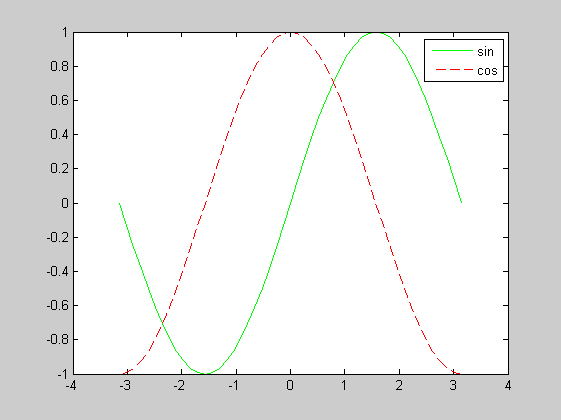
\includegraphics[width=0.5\columnwidth]{sample_figure.png}
\end{center}
\caption{Sin and
Cosine.}
\vskip\baselineskip % Leave a vertical skip below the figure
\label{fig:sample}
\end{figure}

Now, let us cite some studies: one source as \cite{doebelin},  two
sources as \cite{doebelin,exoplanetwebsite} or you may cite three or
more sources as 
\cite{doebelin,exoplanetwebsite,aran2007databaseofnon-manual}.\nocite{
liudissertation} \nocite{paper-IAT-2006-labels}
Observe that they are ordered in the references chapter in the same
order as
they are cited. Let us put a sample table as seen in Table
\ref{table:sample}. Please pay attention that the caption is followed
by a period.

\begin{table}[thbp]
\vskip\baselineskip 
\caption[Sample table]{Sample table.}
\begin{center}
\begin{tabular}{|c|c|c|}\hline
 & \textbf{Header 1}& \textbf{Header 2}\\\hline
\textbf{Row 1} & Bla bla bla& Bla bla bla \\\hline
\textbf{Row 2} & Bla bla bla  & Bla bla bla \\\hline
\end{tabular}
\label{table:sample}
\end{center}
\end{table}



Footnotes should be avoided as possible. If there is an absolute
necessity, footnotes should be used as this.\footnote{Example of a
footnote}

Item lists may be represented as follows:

\begin{itemize}
 \item This is an item. Do not use boldface for the items.
\begin{enumerate}
 \item This is a sub-item. Subsub-items are not allowed.
\end{enumerate}
\item Another item.
\end{itemize}
%  \item 
% \end{enumerate}
Item lists may also be represented as follows:
\begin{enumerate}
 \item This is another enumerated item.
\begin{itemize}
 \item This is another sub-item.
\end{itemize}

\end{enumerate}

\begin{thm}
The solutions of the equation $ax^2+bx+c=0$ with $a\neq 0$ are
$$
x=\frac{-b\pm \sqrt{b^2-4ac}}{2a}
$$
\end{thm}


\begin{proof}
We use the method of completing the square to rewrite $ax^2+bx+c$.
\begin{align*}
ax^2+bx+c&=a\left( x^2 + \frac{b}{a}x+\right)+c \\
  &=a\left( x^2 + \frac{b}{a}x+ \left(\frac{b}{2a}\right)^2
     -\left(\frac{b}{2a}\right)^2 +\right)+c \\
  &=a\left( x+\frac{b}{2a}\right)^2 - 
a\left(\frac{b}{2a}\right)^2+c\\
  &= a\left( x+\frac{b}{2a}\right)^2- \frac{b^2-4ac}{4a}.
\end{align*}
Therefore $ax^2+bx+c=0$ can be rewritten as 
$$
a\left( x+\frac{b}{2a}\right)^2- \frac{b^2-4ac}{4a}=0,
$$
which can in turn  be rearranged as
$$
\left( x+\frac{b}{2a}\right)^2= \frac{b^2-4ac}{4a^2}.
$$
Taking square roots gives
$$
x+\frac{b}{2a}= \frac{\pm \sqrt{b^2-4ac}}{2a}
$$
which implies
$$
x=\frac{-b\pm \sqrt{b^2-4ac}}{2a}
$$
as required.
\end{proof}
Finally, we will put a sample algorithm (PCA algorithm) using the
relevant package in a figure as shown in Figure \ref{alg:pca} and
sample equations.

\begin{figure}[htbp]
\label{alg:pca}
\begin{center}
\framebox[6.0in]{\begin{minipage}[t]{5.9in}
\begin{algorithmic}
\STATE
\STATE \textbf{Require}  $\mathbf{s_i},\ i=1,2,\dots,N$ are normalized
 
\STATE Compute the mean  $\mathbf{\bar{s}}$ using Eq. \ref{eq:mean};
\STATE Form the $N\times2L$ matrix $\mathbf{Q}$ as defined in Eq.
\ref{eq:q};
\IF{ $N < 2\times L$}
\STATE $\mathbf{Q} \Leftarrow \mathbf{Q}^T$ ;
\ENDIF
\STATE Compute the covariance matrix $\mathbf{C}_s$ using Eq.
\ref{eq:cov_matrix};\STATE Decompose $\mathbf{C}_s$
 to its eigenvectors   $\mathbf{e}_k$  and eigenvalues $\lambda_k$
satisfying Eq. \ref{eq:pca};
\IF{ $N < 2\times L$}
\FOR{$k=1$ to $K$}
\STATE $\mathbf{e}_k \Leftarrow \mathbf{Q}\mathbf{e}_k $ ;
\STATE $\mathbf{e}_k \Leftarrow \mathbf{e}_k/||\mathbf{e}_k|| $
(normalization);
\ENDFOR
\ENDIF
\STATE
\end{algorithmic}
\end{minipage}}
\end{center}
\caption[Principal Component Analysis Algorithm]{Principal Component
Analysis Algorithm.}
% \vskip
\end{figure}

\begin{align} 
\mathbf{\bar{s}} & =\frac{1}{N} \sum_{i=1}^N \mathbf{s}_i
\label{eq:mean}   
\\
\mathbf{Q} & =\left[ 
\begin{array}{cccc} 
 \mathbf{s}_1  - \mathbf{\bar{s}} & \mathbf{s}_2 - \mathbf{\bar{s}} &
\cdots & \mathbf{s}_N  - \mathbf{\bar{s}}
\end{array}
\right]_{2L\times N }
\label{eq:q}
\\ 
\mathbf{C}_s & =\frac{1}{N} \mathbf{Q}^T \mathbf{Q}
\label{eq:cov_matrix}
\end{align}

\begin{equation}
    \mathbf{C}_s \mathbf{e}_k = \lambda_k \mathbf{e}_k
    \label{eq:pca}
\end{equation}

\subsection{Example of First Subheadings}
Some text here
\subsubsection{Example of Second Subheadings}
Some text here too.
\chapter{CONCLUSION}
\label{chapter:conclusion}

The conclusions of the thesis should come
here.
% \nocite{NewEntry1,NewEntry2,NewEntry3,NewEntry4,NewEntry5,
% NewEntry6,
% NewEntry7,NewEntry8,NewEntry9,NewEntry10,NewEntry11,NewEntry12}

%\cite{*}
\bibliographystyle{styles/fbe_tez_v11}
\bibliography{references}

\appendix
\chapter{APPLICATION}
The appendices start here.

\end{document}